\section{A Case Study: VLIW Hardware/Software Design Space}
\label{sec:ee}
In this subsection we evaluating the behavior of the proposed approach
using a parameterized Very Long Instruction
Word (VLIW) architecture~\cite{kathail_tr00} as a testbed. The same philosophy
behind a VLIW system makes it a natural choice for several reasons:
\begin{itemize}
\item{Multi-Objective trade-offs}: these architectures let designers
easily trade between power, energy and performances~\cite{}, leading
to Pareto sets whose extension is an ideal ground for testing the
proposed Parameters space representation.
\item{Compiler awareness}: Instruction Level Parallelism (ILP)
constitutes the key feature to enable the multi-objective trade-offs
of the point above. It is statically obtained by the compiler which
performs code trasformations being aware of the underlying hardware
configuration.  This tight hardware/software dependence, makes the
VLIW scenario more suitable for investigating hardly predictable
hardware/software interactions, especially when compared to
architectures where, in order to preserve binary compatibility,
software generation processes are independent from the hardware that
will execute it.

System parameters can be classified in three main categories:
\emph{processor}, \emph{memory sub-system} and \emph{compiling options}. 
The first is directly related to the VLIW core and includes the size
of the register files and the number of functional
units for each type of opera. In particular, five different types of register files can be identified:
GPR (32-bit registers for integers), FPR (64-bit registers for
floating point values) PR (1-bit registers used to store the Boolean
values of predicated instructions), BTR (64-bit registers containing
information about possible future branches) and CR (32-bit control
registers containing information about the internal state of the
processor). The functional units involved are: \emph{Integer units},
\emph{floating point units}, \emph{memory units} (associated with
load/store operations) and \emph{branch units} (associated with branch
operations). With respect to the memory sub-system, the parameters
include \emph{size}, \emph{associativity} and
\emph{block size} for each of the three caches: First-level data cache
(L1D), first-level instruction cache (L1I) and second-level unified
cache (L2U).

Further, a set of the most impacting compilation parameters has been
selected and included in the configuration space:
\begin{itemize}
\item{tcc\_region}: Specifies the scope of action of the compiler and the type
of code transformation involved (basic block, super block and hyper
block) 
\item {max\_unroll\_allowed}: The number of unroll iterations allowed
\item{regroup\_only}: Avoids inlining 
\item{do\_classic\_opti}: A set of classical optimization, not VLIW related,
such as common expression removal 
\item{do\_prepass\_scalar\_scheduling}: Performs a schedule before
forming regions 
\item{do\_postpass\_scalar\_scheduling}: Performs a schedule after the region formation 
do\_modulo\_scheduling & Modular scheduling 
\item{memvr\_profiled}: Performs a memory-dependencies profiling 
\end{itemize}

\subsection{Evaluation Metrics}

The results presented in the next section compare PS against a widely
adpted Multi-objective Genetic Algorithm~\cite{}. At best of our
knowledge, genetic approaches
still represent the best compromise between efficiency (i.e. time
required for exploration) and accuracy of the reported Paret Sets. Of
course mono-objective approaches have been
deliberately excluded from this analysis. Other
approaches~\cite{dep} that make use of some a-priori knowledge about the
role and meaning of each parameter have been also excluded, since our
aim is evaluate the capacity of the strategy to focus on interesting
parameter regions without any external judgement or help based on
euristics.  Finally, it should be pointed
out that in this introductory work we explicitly focus on TODO
remainding to works like~\cite{} for a detailed analysis of other
similar multi-objective strategies.

The class of benchmark being considered is representative of some common
frequently running application kernels in an embedded multimedia
environment. Table~\ref{tab:bench} shows the set of applications
chosen along with a brief description.
\begin{table}
	\centering
	\caption{Benchmarks}
	\label{tab:bench}
	\begin{tabular}{ll}
	\hline
	\multicolumn{1}{c}{Benchmark} & \multicolumn{1}{c}{Application} \\
	\hline
	Alloca\_test & Memory array allocation test \\
	Bmm & Matrices multiplication and elements sum \\
	Fir\_int & Finite impulse response \\
	Fib & Fibonacci series \\
	Mm & Floating point matrices multiplication \\
	Wave & Wavefront computation \\
	\hline
	\end{tabular}
\end{table}
%------------------------------------------------------------------------------

\section{Results}

Each data set is obtained evaluation a 1,000 randomly chosen point of
the configuration space. In particular, two different scenarios have
been considered: the first one, referred as \emph{Variable Compilation
Profile (VCP)}, includes all compilation parameters described
in the Table~\ref{tab:compiler}; a second scenario, \emph{Fixed
Compilation Profile (FCP)}, which excludes any of those parameters
exploring all the remaining hardware aspects of the architecture as
described in Section~\ref{subsec:arch}.

Figures~\ref{fig:pareto_fronts_100} and~\ref{fig:pareto_fronts}
respectively show the visited configurations and the
Pareto fronts found for both FCP and VCP scenarios for different
application benchmarks. How it can be observed, VCP solutions
are on average  more widely and evenly distributed over the objective
space as compared to those found for the FCP case.


\begin{figure}
  \centering
  \begin{tabular}{cc}
    \includegraphics[width=0.45\textwidth]{pictures/100bmm.eps} & \includegraphics[width=0.45\textwidth]{pictures/100fir_int.eps} \\
    \includegraphics[width=0.45\textwidth]{pictures/100mm.eps} & \includegraphics[width=0.45\textwidth]{pictures/100fib.eps} \\
    \includegraphics[width=0.45\textwidth]{pictures/100alloca_test.eps} & \includegraphics[width=0.45\textwidth]{pictures/100wave.eps}
  \end{tabular}
  \caption{Pareto fronts found by PS and GA for a fixed budget of 100 configurations.}
  \label{fig:pareto_fronts_100}
\end{figure}

\begin{figure}
  \centering
  \begin{tabular}{cc}
    \includegraphics[width=0.45\textwidth]{pictures/bmm.eps} & \includegraphics[width=0.45\textwidth]{pictures/fir_int.eps} \\
    \includegraphics[width=0.45\textwidth]{pictures/mm.eps} & \includegraphics[width=0.45\textwidth]{pictures/fib.eps} \\
    \includegraphics[width=0.45\textwidth]{pictures/alloca_test.eps} & \includegraphics[width=0.45\textwidth]{pictures/wave.eps}
  \end{tabular}
  \caption{Pareto fronts found by PS and GA for a fixed budget of 500 configurations.}
  \label{fig:pareto_fronts}
\end{figure}

Let us now analyse the Pareto fronts from a quantitative viewpoint. We
consider two metrics, namely, the \emph{variation range} and the
\emph{average normalised absolute dispersion error}. For a given
objective, the variation range represents the ratio between the
maximum and the minimum value observed for that objective. A
comparison between the variation range for different benchmarks
between a FCP and a VCP exploration for both power dissipation and
execution time is shown in Fig.~\ref{fig:variation_range}. As it can
be observed, the VCP exploration provides solutions which fall on a
range that is, on average, 23\% and 40\% wider than that provided by a
FCP exploration for power dissipation and execution time,
respectively.
\begin{figure}
  \centering
  \begin{tabular}{c}
    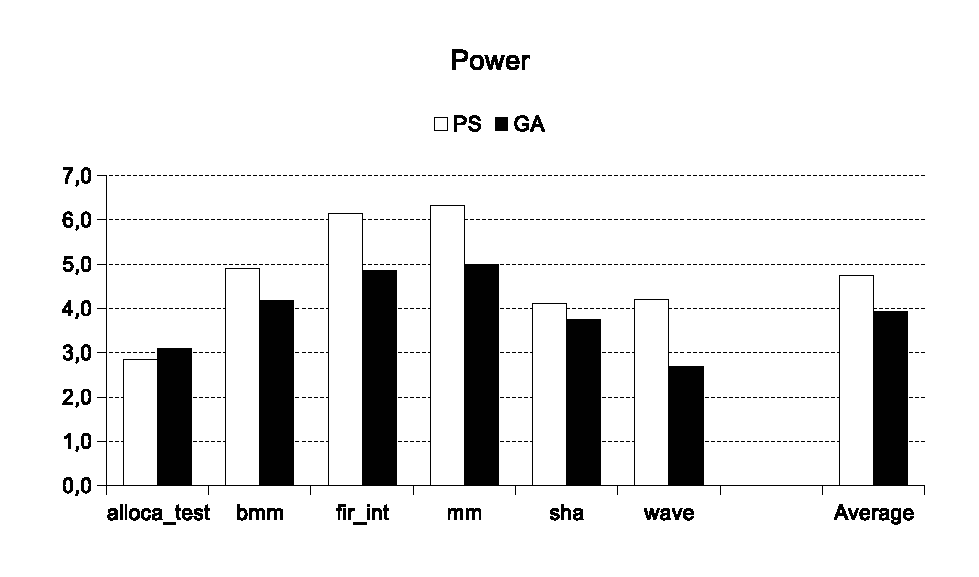
\includegraphics[width=0.7\textwidth]{pictures/variation_power.eps} \\
    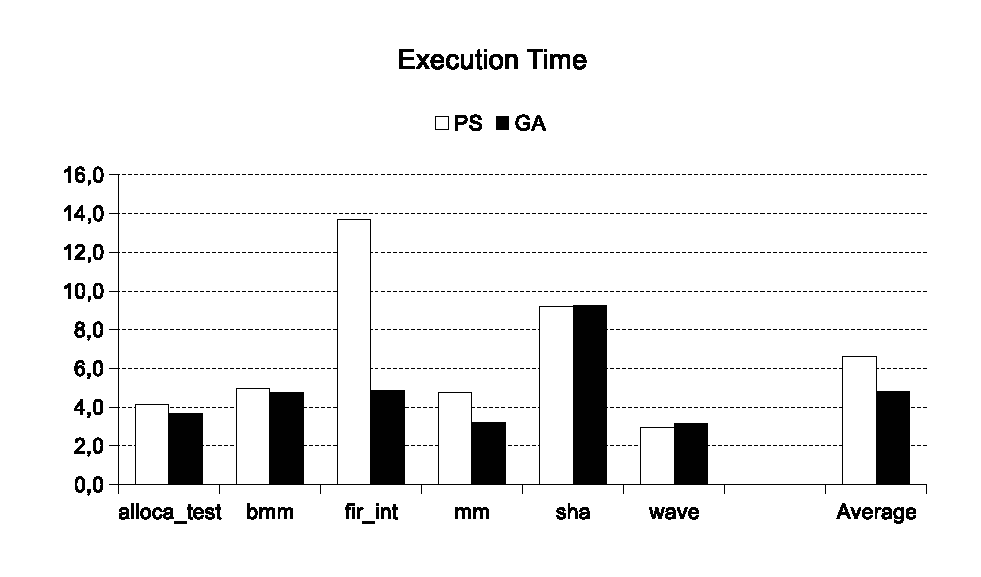
\includegraphics[width=0.7\textwidth]{pictures/variation_etime.eps}
  \end{tabular}
  \caption{Variation range for different benchmarks between a FCP and
    a VCP exploration for power dissipation and execution time.}
  \label{fig:variation_range}
\end{figure}


The average normalised absolute dispersion error measures
the average absolute difference between the distribution of points in
the objective space and an ideal distribution in which the points are
uniformly distributed over the objective space. Formally, let $O$ be
the image, in the objective space, of the configurations visited by
the design space exploration. The generic element of $O$ (\ie, a
solution) is a pair $(p,t)$ where $p$ and $t$ are the average power
and execution time, respectively. The two-dimensional objective space
is then partitioned by a $M_x \times M_y$ mesh. For each tile $T_i,
\ i=1, 2, \ldots, M_xM_y$ of the mesh, let $N_i$ be the number
of points in $O$ which fall in $T_i$. The average absolute error, $E_i$, for
$T_i$ is the absolute value of the difference between $N_i$ and the
ideal number of solutions, $\overline{N}$, which should fall in $T_i$
in case of uniform distribution. Such $\overline{N}$ can be simply
computed as the ratio between the cardinality of $O$ and the number of
tiles. Thus,
\[ E_i = |N_i - \overline{N}|, \]
where $\overline{N} = |O| / (M_x M_y)$. The average
normalised absolute dispersion error ($ANADE$) is the average of $E_i$
normalised to the maximum absolute error $E_{max}$:
\[ ANADE = \frac{\sum_{i=1}^{M_xM_y} E_i/(M_xM_y)}{E_{max}}, \]
where $E_{max}$ can be computed as the average absolute error in the worst
case in which all the solutions fall in a single tile:
\[ E_{max} = \frac{(M_x M_y - 1) \overline{N} + |\overline{N} -
    |O|| }{M_x M_y}. \] 

Fig.~\ref{fig:dispersion} shows the average normalised absolute
dispersion errors for different benchmarks for FCP and VCP
exploration. As it can be observed, VCP exploration reduces the
dispersion error on average by 20\% as compared to a FCP exporation.
\begin{figure}
  \centering
  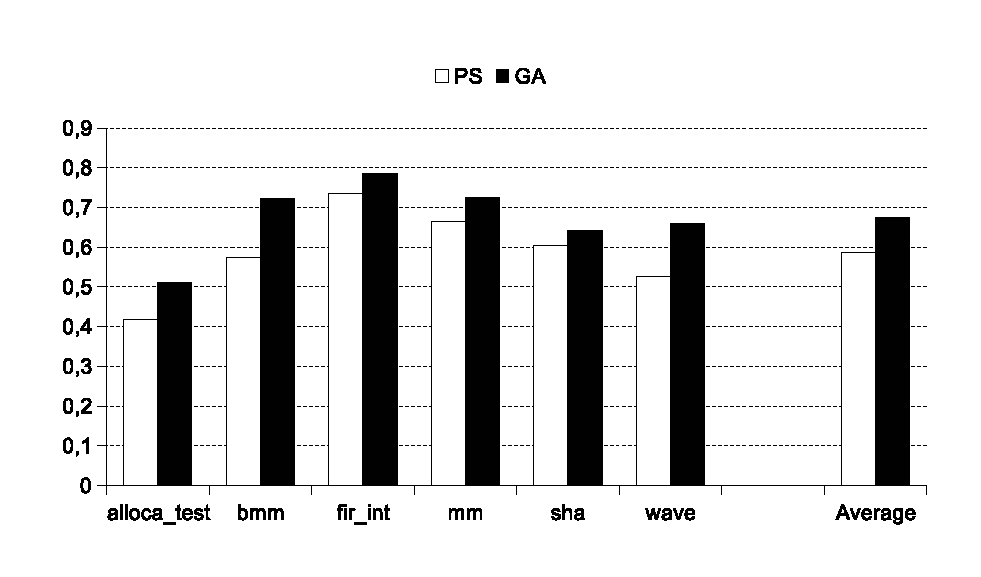
\includegraphics[width=0.7\textwidth]{pictures/dispersion.eps} \\
  \caption{Average normalised absolute dispersion errors for different
    benchmarks for FCP and VCP exploration.}
  \label{fig:dispersion}
\end{figure}
